\documentclass[a4paper,12pt]{memoir}

\usepackage{hyperref}
\usepackage{marvosym}
\usepackage{fontawesome}

\hypersetup{
    colorlinks=true,
    linkcolor=black,
    filecolor=black,
    urlcolor=black,
}

%%%%%%%%%%%%%%%%%%%%%%%%%%%%%%%%%%%%%%%%%
% Wenneker Resume/CV
% Structure Specification File
% Version 1.1 (19/6/2016)
%
% This file has been downloaded from:
% http://www.LaTeXTemplates.com
%
% Original author:
% Frits Wenneker (http://www.howtotex.com) with extensive modifications by 
% Vel (vel@latextemplates.com)
%
% License:
% CC BY-NC-SA 3.0 (http://creativecommons.org/licenses/by-nc-sa/3.0/)
%
%%%%%%%%%%%%%%%%%%%%%%%%%%%%%%%%%%%%%%%%%

%----------------------------------------------------------------------------------------
%	PACKAGES AND OTHER DOCUMENT CONFIGURATIONS
%----------------------------------------------------------------------------------------

\usepackage{XCharter} % Use the Bitstream Charter font
\usepackage[utf8]{inputenc} % Required for inputting international characters
\usepackage[T1]{fontenc} % Output font encoding for international characters

\usepackage[top=1cm,left=1cm,right=1cm,bottom=1cm]{geometry} % Modify margins

\usepackage{graphicx} % Required for figures

\usepackage{flowfram} % Required for the multi-column layout

\usepackage{url} % URLs

\usepackage[usenames,dvipsnames]{xcolor} % Required for custom colours

\usepackage{tikz} % Required for the horizontal rule

\usepackage{enumitem} % Required for modifying lists
\setlist{noitemsep,nolistsep} % Remove spacing within and around lists

\setlength{\columnsep}{\baselineskip} % Set the spacing between columns

% Define the left frame (sidebar)
\newflowframe{0.2\textwidth}{\textheight}{0pt}{0pt}[left]
\newlength{\LeftMainSep}
\setlength{\LeftMainSep}{0.2\textwidth}
\addtolength{\LeftMainSep}{1\columnsep}
 
% Small static frame for the vertical line
\newstaticframe{1.5pt}{\textheight}{\LeftMainSep}{0pt}
 
% Content of the static frame with the vertical line
\begin{staticcontents}{1}
\hfill
\tikz{\draw[loosely dotted,color=RoyalBlue,line width=1.5pt,yshift=0](0,0) -- (0,\textheight);}
\hfill\mbox{}
\end{staticcontents}
 
% Define the right frame (main body)
\addtolength{\LeftMainSep}{1.5pt}
\addtolength{\LeftMainSep}{1\columnsep}
\newflowframe{0.7\textwidth}{\textheight}{\LeftMainSep}{0pt}[main01]

\pagestyle{empty} % Disable all page numbering

\setlength{\parindent}{0pt} % Stop paragraph indentation

%----------------------------------------------------------------------------------------
%	NEW COMMANDS
%----------------------------------------------------------------------------------------

\newcommand{\userinformation}[1]{\renewcommand{\userinformation}{#1}} % Define a new command for the CV user's information that goes into the left column

\newcommand{\cvheading}[1]{{\Huge\bfseries\color{RoyalBlue} #1} \par\vspace{.6\baselineskip}} % New command for the CV heading
\newcommand{\cvsubheading}[1]{{\Large\bfseries #1} \bigbreak} % New command for the CV subheading

\newcommand{\Sep}{\vspace{1em}} % New command for the spacing between headings
\newcommand{\SmallSep}{\vspace{0.5em}} % New command for the spacing within headings

\newcommand{\aboutme}[2]{ % New command for the about me section
\textbf{\color{RoyalBlue} #1}~~#2\par\Sep
}
	
\newcommand{\CVSection}[1]{ % New command for the headings within sections
{\Large\textbf{#1}}\par
\SmallSep % Used for spacing
}

\newcommand{\CVItem}[2]{ % New command for the item descriptions
\textbf{\color{RoyalBlue} #1}\par
#2
\SmallSep % Used for spacing
}

\newcommand{\bluebullet}{\textcolor{RoyalBlue}{$\circ$}~~} % New command for the blue bullets


%!TEX root = ./cv.tex

% Personal Info

\usepackage{tikz}

\userinformation{
	\begin{flushright}
		\begin{tikzpicture}
			\clip (0,0)  circle (2cm) ;
			\node {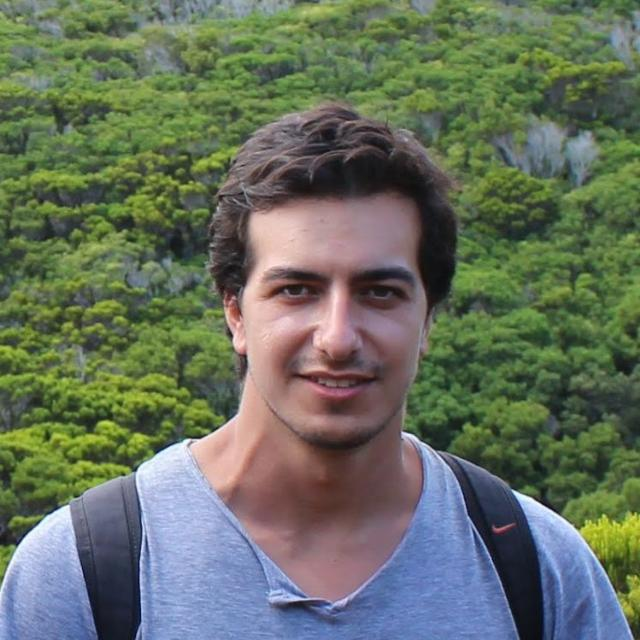
\includegraphics[width=4cm]{photo3.jpeg}}; 
		\end{tikzpicture}
		%
\includegraphics[width=0.8\columnwidth]{photo2.jpeg}\\[\baselineskip]

		\small

		André Pascoal Bento \\
		%\Letter~\href{mailto:andre.pascoal.bento@gmail.com}{andre.pascoal.bento@gmail.com} \\
		\Letter~\href{mailto:apbento@dei.uc.pt}{apbento@dei.uc.pt} \\
		\Mobilefone~(+351)~910~349~466 \\
		%\Telefon~(+351)~231~455~067 \\ 
		\faLinkedin~\href{https://www.linkedin.com/in/andre-bento/?locale=en_US}{andre-bento}
		\faGithub~\href{https://github.com/andrepbento}{andrepbento}
		\faGoogle~\href{https://scholar.google.com/citations?user=9Yl9gBwAAAAJ&hl=en}{Schollar}

		\Sep

		\textbf{Address} \\
		R. Lourenço Chaves de Almeida, Lote 2, 2.D \\
		Coimbra, 3000-249 \\
		Portugal

		\Sep

		\textbf{Communication skills} \\
		Portuguese (native) \\
		English (advanced) \\
		French (intermediate) \\
		Spanish (intermediate)

		\vfill
	\end{flushright}
}


\begin{document}

\userinformation

\framebreak

\cvheading{André Bento}

\cvsubheading{PhD Student @ CISUC | Assistant Professor @ University of Coimbra}

\aboutme{About}{
    André Bento is a researcher at the Centre for Informatics and Systems at the University of Coimbra.
    He is also a PhD student in Informatics Engineering, an invited professor and participates in the project AESOP -- Autonomic Service Operation.
    He received his BSc degree from the Coimbra Institute of Engineering and his MSc degree from the University of Coimbra, both in Informatics Engineering.
    Besides studying and working, André Bento is a regular swimmer, and enjoys cycling, running and long walks in nature.
    As an enthusiast of distributed systems and cloud-based solutions, he is constantly looking for opportunities to improve and learn new methods and technologies.
}

\CVSection{Education}

\CVItem{2019 - Present, University of Coimbra}{PhD in Information Science and Technology}

\CVItem{2017 - 2019, University of Coimbra}{MSc in Informatics Engineering\\\emph{Thesis: Observing and Controlling Performance in Microservices}}

\CVItem{2014 - 2017, Coimbra Institute of Engineering (ISEC)}{BSc in Informatics Engineering}

\Sep

\CVSection{Experience}

\CVItem{Sep 2021 - Present, \textit{Invited Professor}, University of Coimbra}{
    Teaching practical laboratory classes on Distributed systems and Systems integration.
}

\CVItem{Sep 2019 - Present, \textit{Researcher}, CISUC - Centre for Informatics and Systems (University of Coimbra)}{
    Research methods and techniques to improve the availability and reliability of microservices using anomaly detection and root-cause analysis.\\
    Working with technologies such as Kubernetes, Terraform, Ansible, AWS, Docker, Istio, Grafana, Prometheus, Jaeger, Kiali, and others.
}

\CVItem{Sep 2018 - Jul 2019, \textit{Research Intern}, CISUC - Centre for Informatics and Systems (University of Coimbra)}{
    Researched Microservices, Observability and Performance Monitoring using Metrics, Logs and Distributed Tracing.
}

\CVItem{Feb 2017 - Jul 2017, \textit{Software Engineer Intern}, WIT Software, S.A.}{
    Developed a Mobile AR Prototype with digital filters and image manipulation features, focusing on enhanced user content creation, e.g., Selfies, Stickers, Photo Effects/Filters, Emojis and Drawing, in an exploratory Android and iOS project.
}

\CVItem{Oct 2016 - Jun 2017, \textit{Scratch Teacher Assistant}, CASPAE 10}{
    Taught problem-solving techniques using the Scratch programming language to children attending the 3rd and 4th grades of primary school.
}

\Sep

\clearpage

\userinformation

\framebreak


\CVItem{Nov 2015 - Mar 2016, \textit{Math Applied to Engineer Teacher -- Volunteer}, CeAMatE}{
    Taught mathematics to pre-degree, CTeSP and Engineering students.
}

\CVItem{Feb 2013 - Jul 2013, \textit{Accountant Technician Intern}, Caixa de Crédito Agrícola Mútuo de Cantanhede e Mira - C.R.L.}{
    Bank accountant, bank organization and bank day-to-day work.
}

\Sep

%!TEX root = ../cv.tex

% Interests

\CVSection{Interests}

\CVItem{Professional}{Microservices, Cloud computing, Tracing, Monitoring, Data analysis,\\Machine learning, Programming languages and Software development}

\CVItem{Personal}{Travelling, Swimming, Trekking, Long walks, Kayak and Canoeing \\Having fun with family and friends}


\end{document}
